\chapter{Scenario Projection}
\label{app:scenario-projection}

\begin{figure}[htbp]
\centering
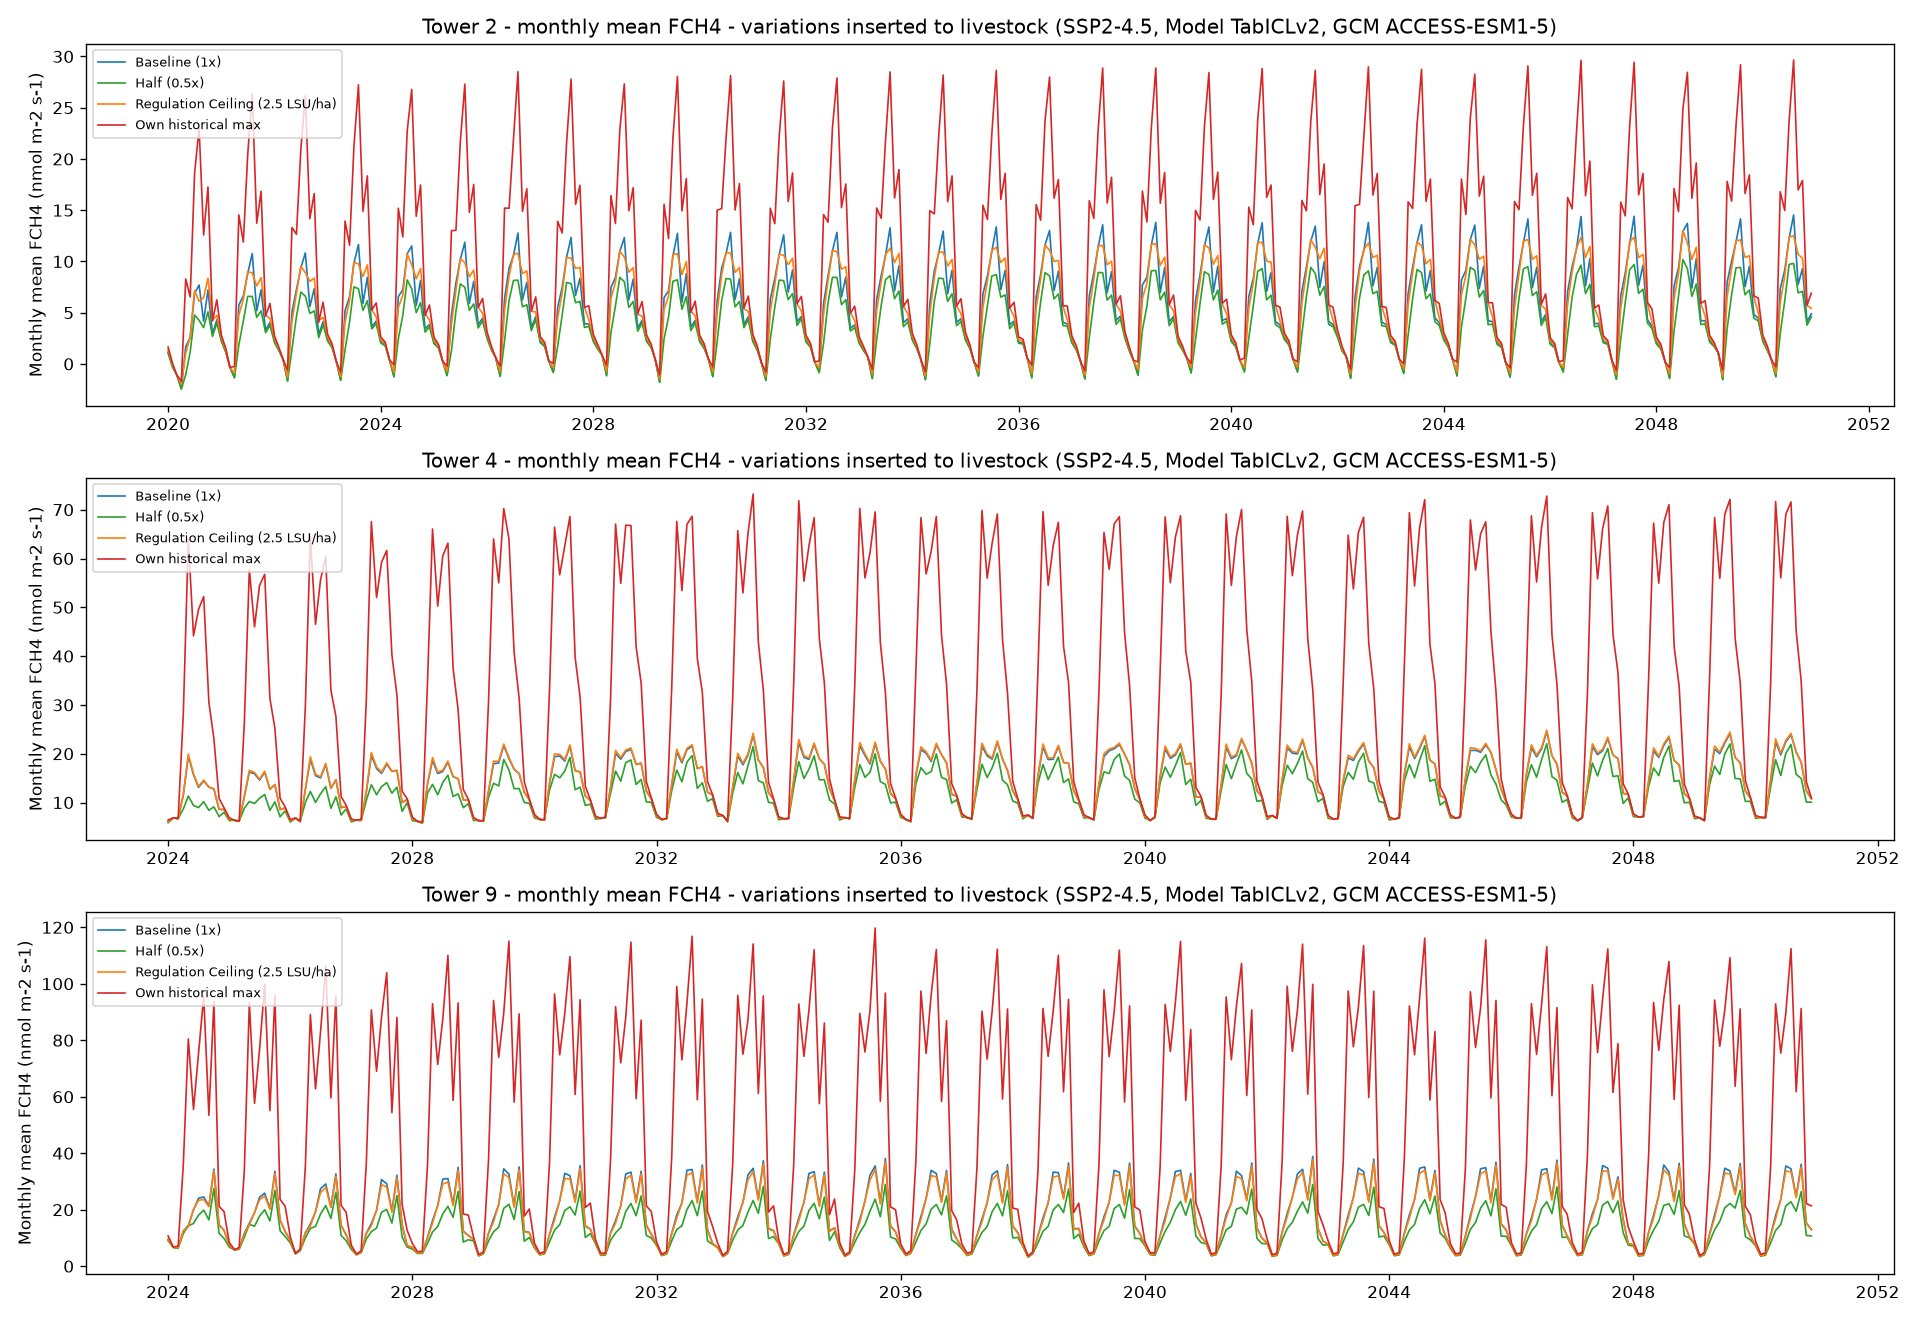
\includegraphics[width=\textwidth]{Figures/ch6_livestock_ladder_trajectory_ssp245.png}
\caption{Monthly mean FCH\textsubscript{4} (nmol~m\textsuperscript{-2}~s\textsuperscript{-1}) at T2, T4 and T9 under SSP2-4.5 for the livestock-density ladder -- baseline, half-density,
government-reference and own-historical-maximum (all-species) -- for a single illustrative
trajectory (restricted model, GCM ACCESS-ESM1-5, realisation~1). Table~\ref{tab:livestock_scenario_results}
reports the mean annual percentage change, averaged across all five GCMs and ten realisations per
GCM.}
\label{fig:app_sp_livestock_trajectory_ssp245}
\end{figure}

\begin{figure}[htbp]
\centering
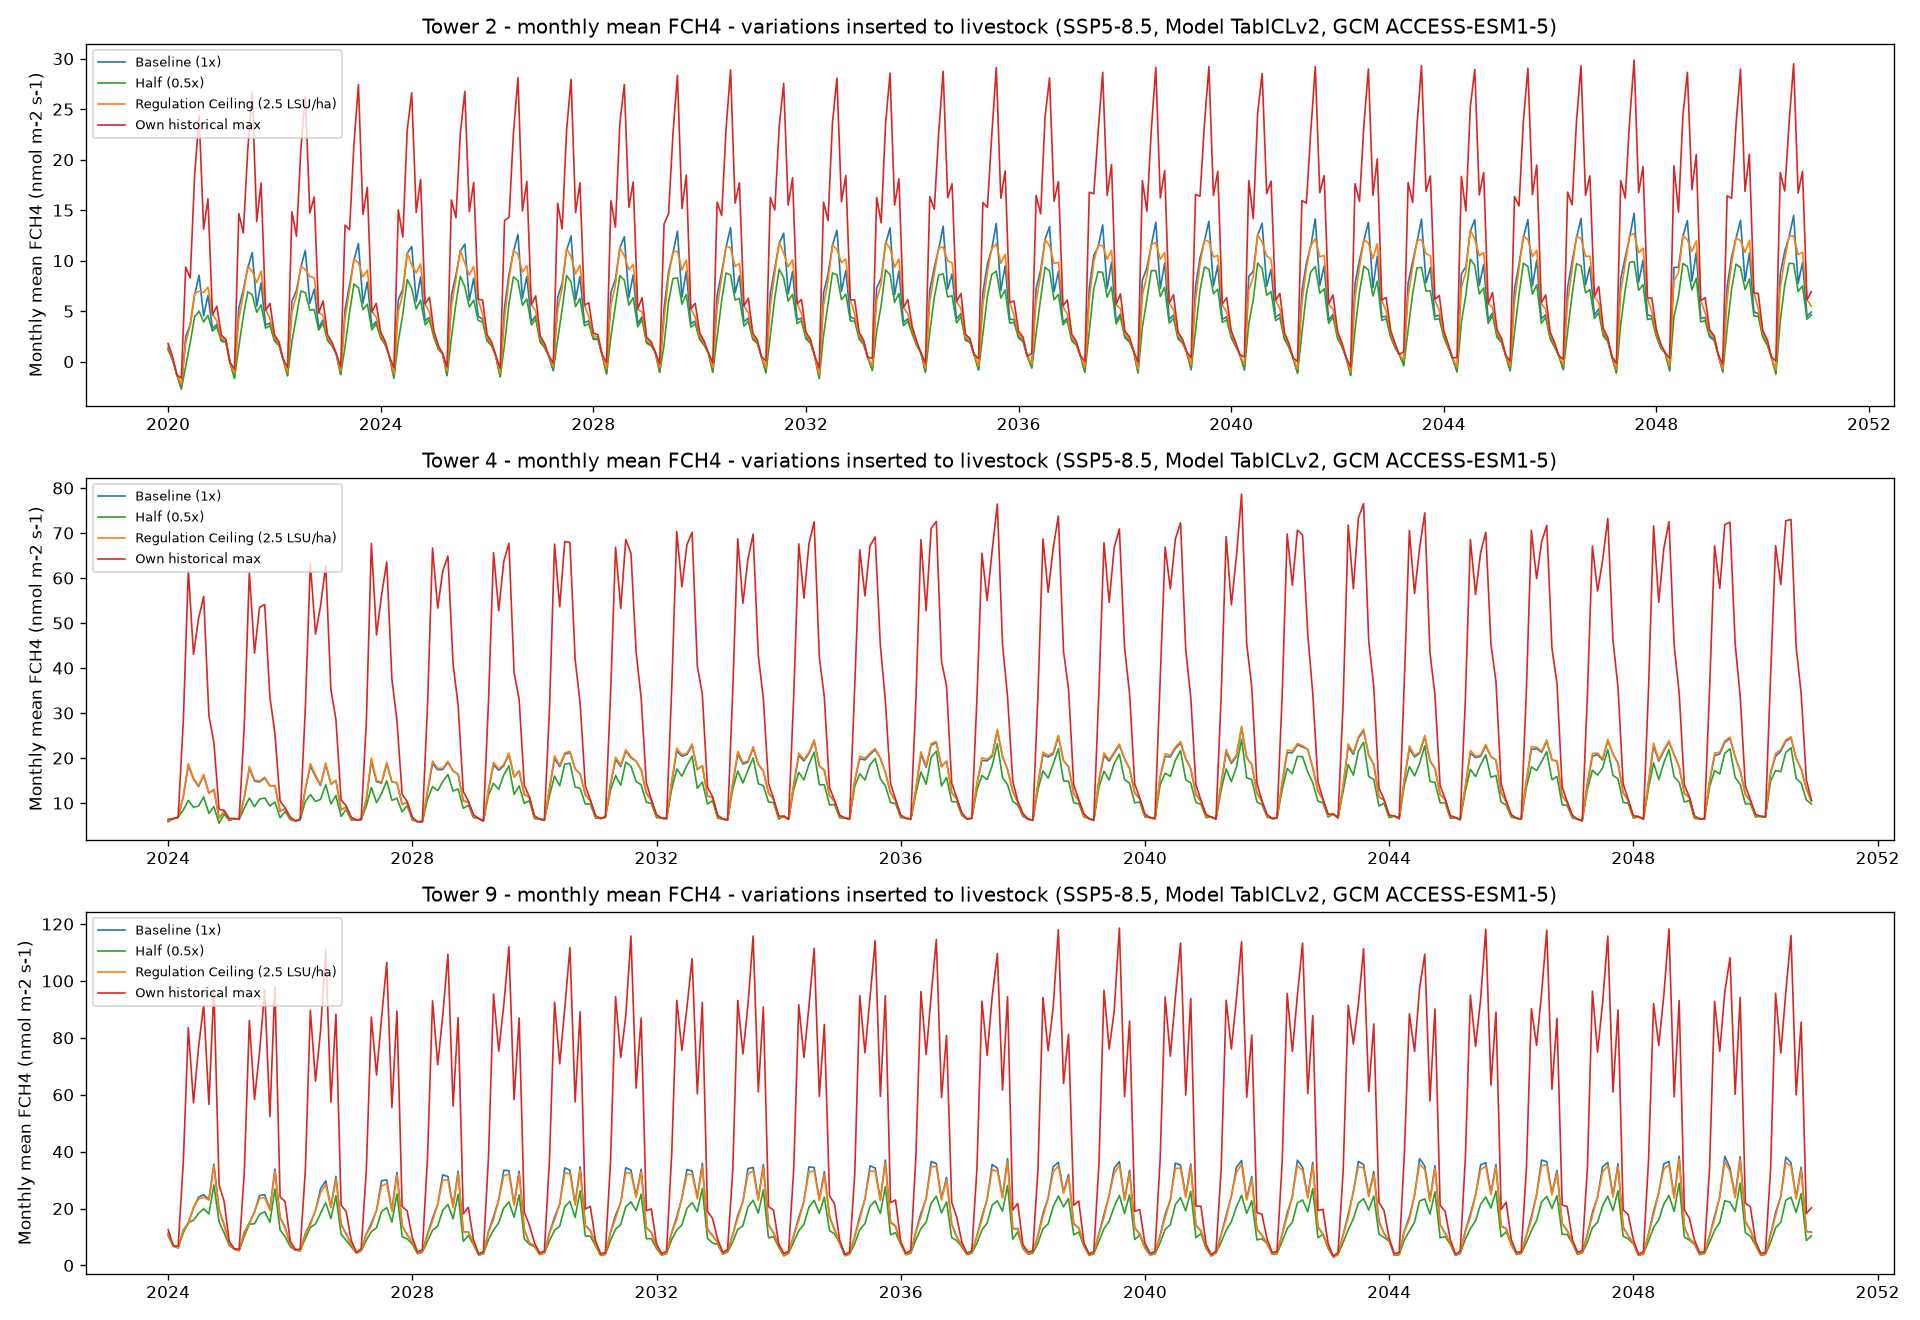
\includegraphics[width=\textwidth]{Figures/ch6_livestock_ladder_trajectory_ssp585.png}
\caption{As Figure~\ref{fig:app_sp_livestock_trajectory_ssp245}, under SSP5-8.5. The near-identical
trajectories under both pathways illustrate Table~\ref{tab:livestock_scenario_results}'s finding
that the SSP pathway itself makes almost no difference to the livestock-density response.}
\label{fig:app_sp_livestock_trajectory_ssp585}
\end{figure}

\FloatBarrier

\begin{figure}[htbp]
\centering
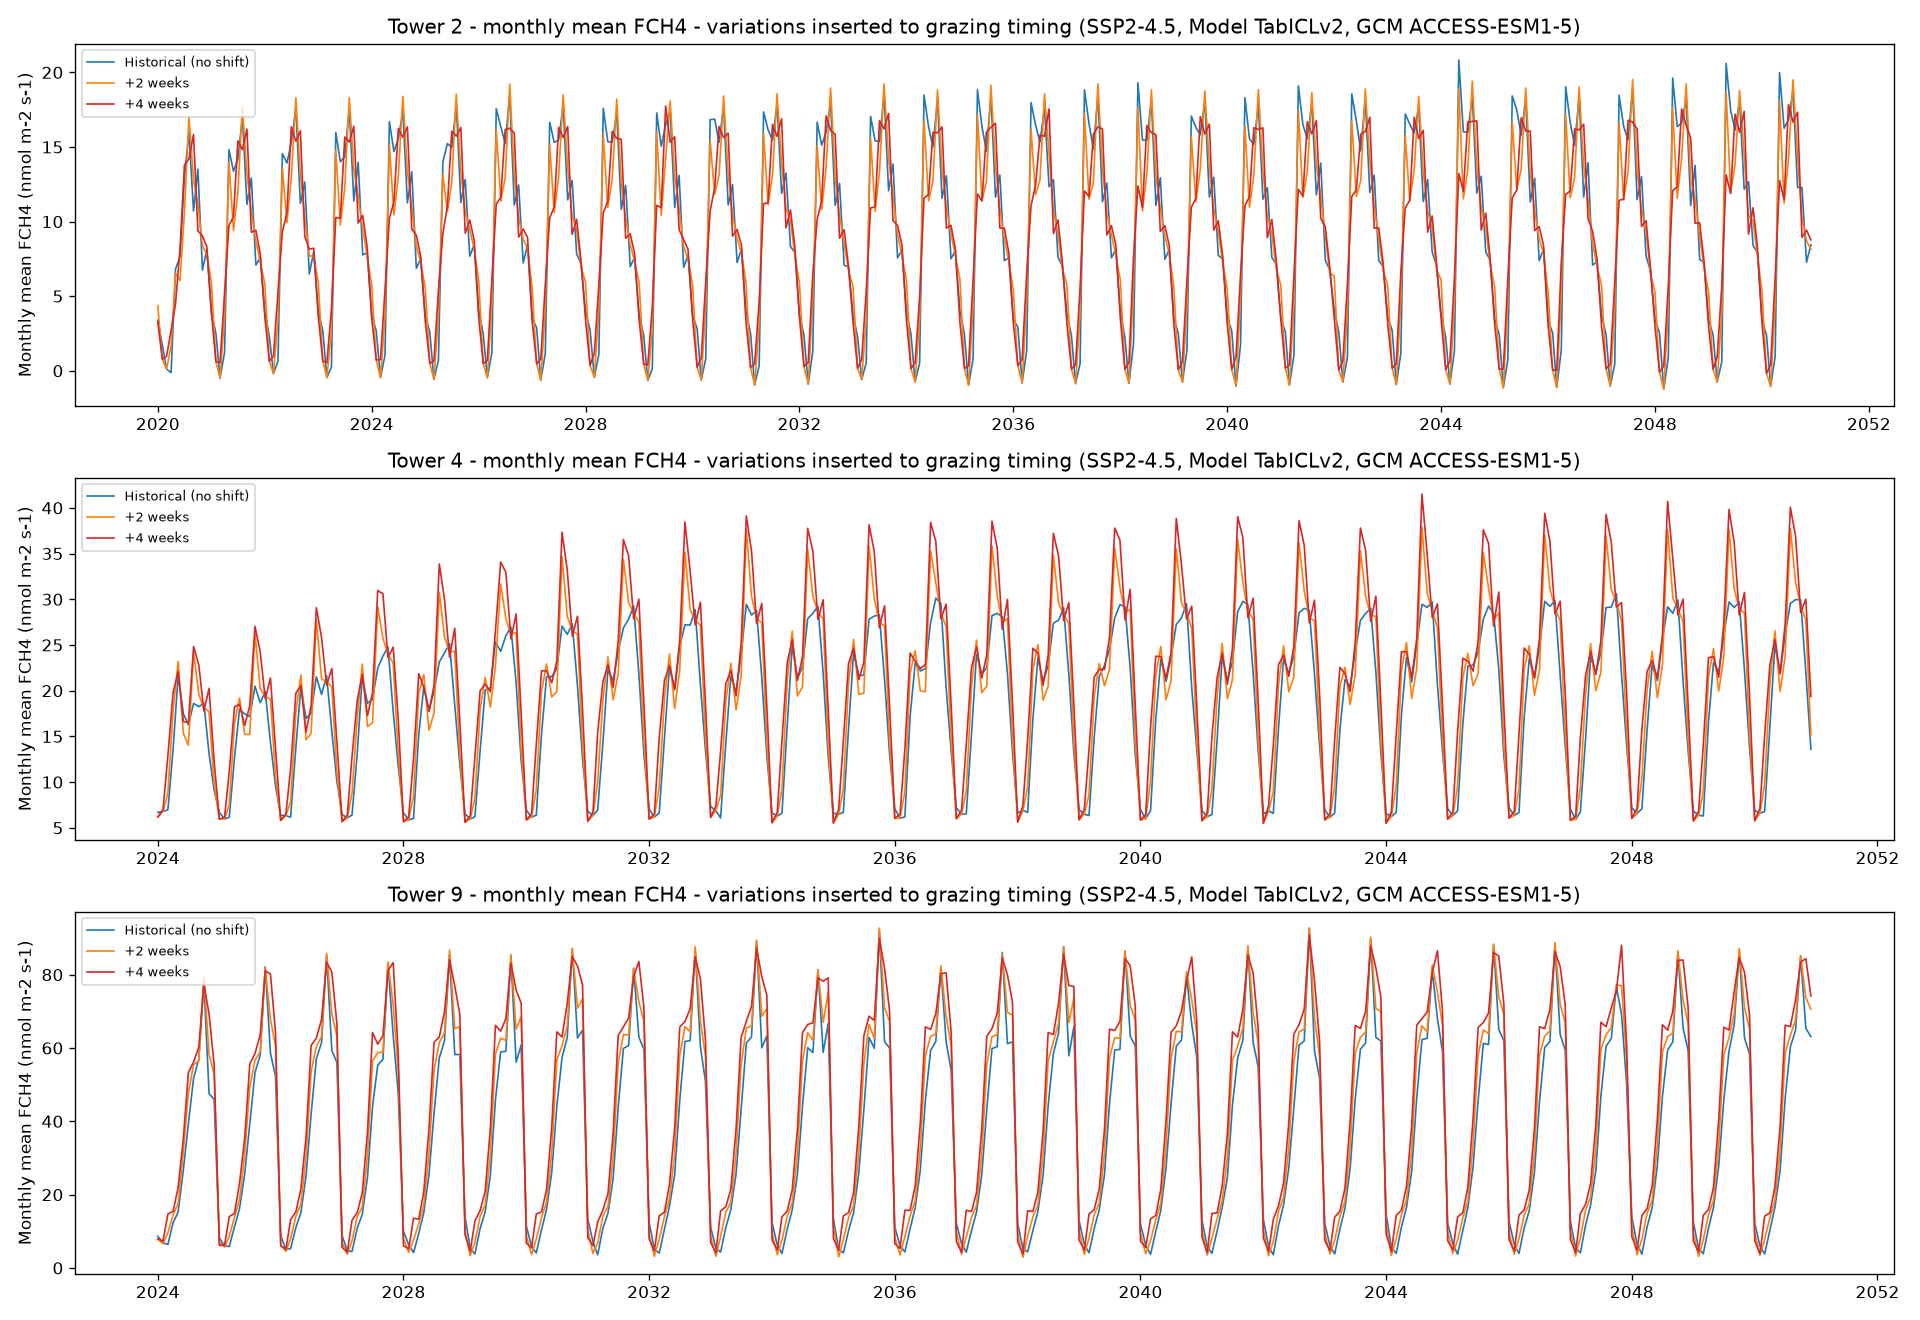
\includegraphics[width=\textwidth]{Figures/ch6_grazing_trajectory_ssp245.png}
\caption{Monthly mean FCH\textsubscript{4} (nmol~m\textsuperscript{-2}~s\textsuperscript{-1}) at T2, T4 and T9 under SSP2-4.5 for the historical grazing-timing baseline and its $+2$-week
and $+4$-week shift perturbations, for a single illustrative trajectory (restricted model, GCM
ACCESS-ESM1-5, realisation~1). Table~\ref{tab:management_scenario_results} reports the mean
annual percentage change for the $+4$-week shift only, averaged across all five GCMs and ten
realisations per GCM.}
\label{fig:app_sp_grazing_trajectory_ssp245}
\end{figure}

\begin{figure}[htbp]
\centering
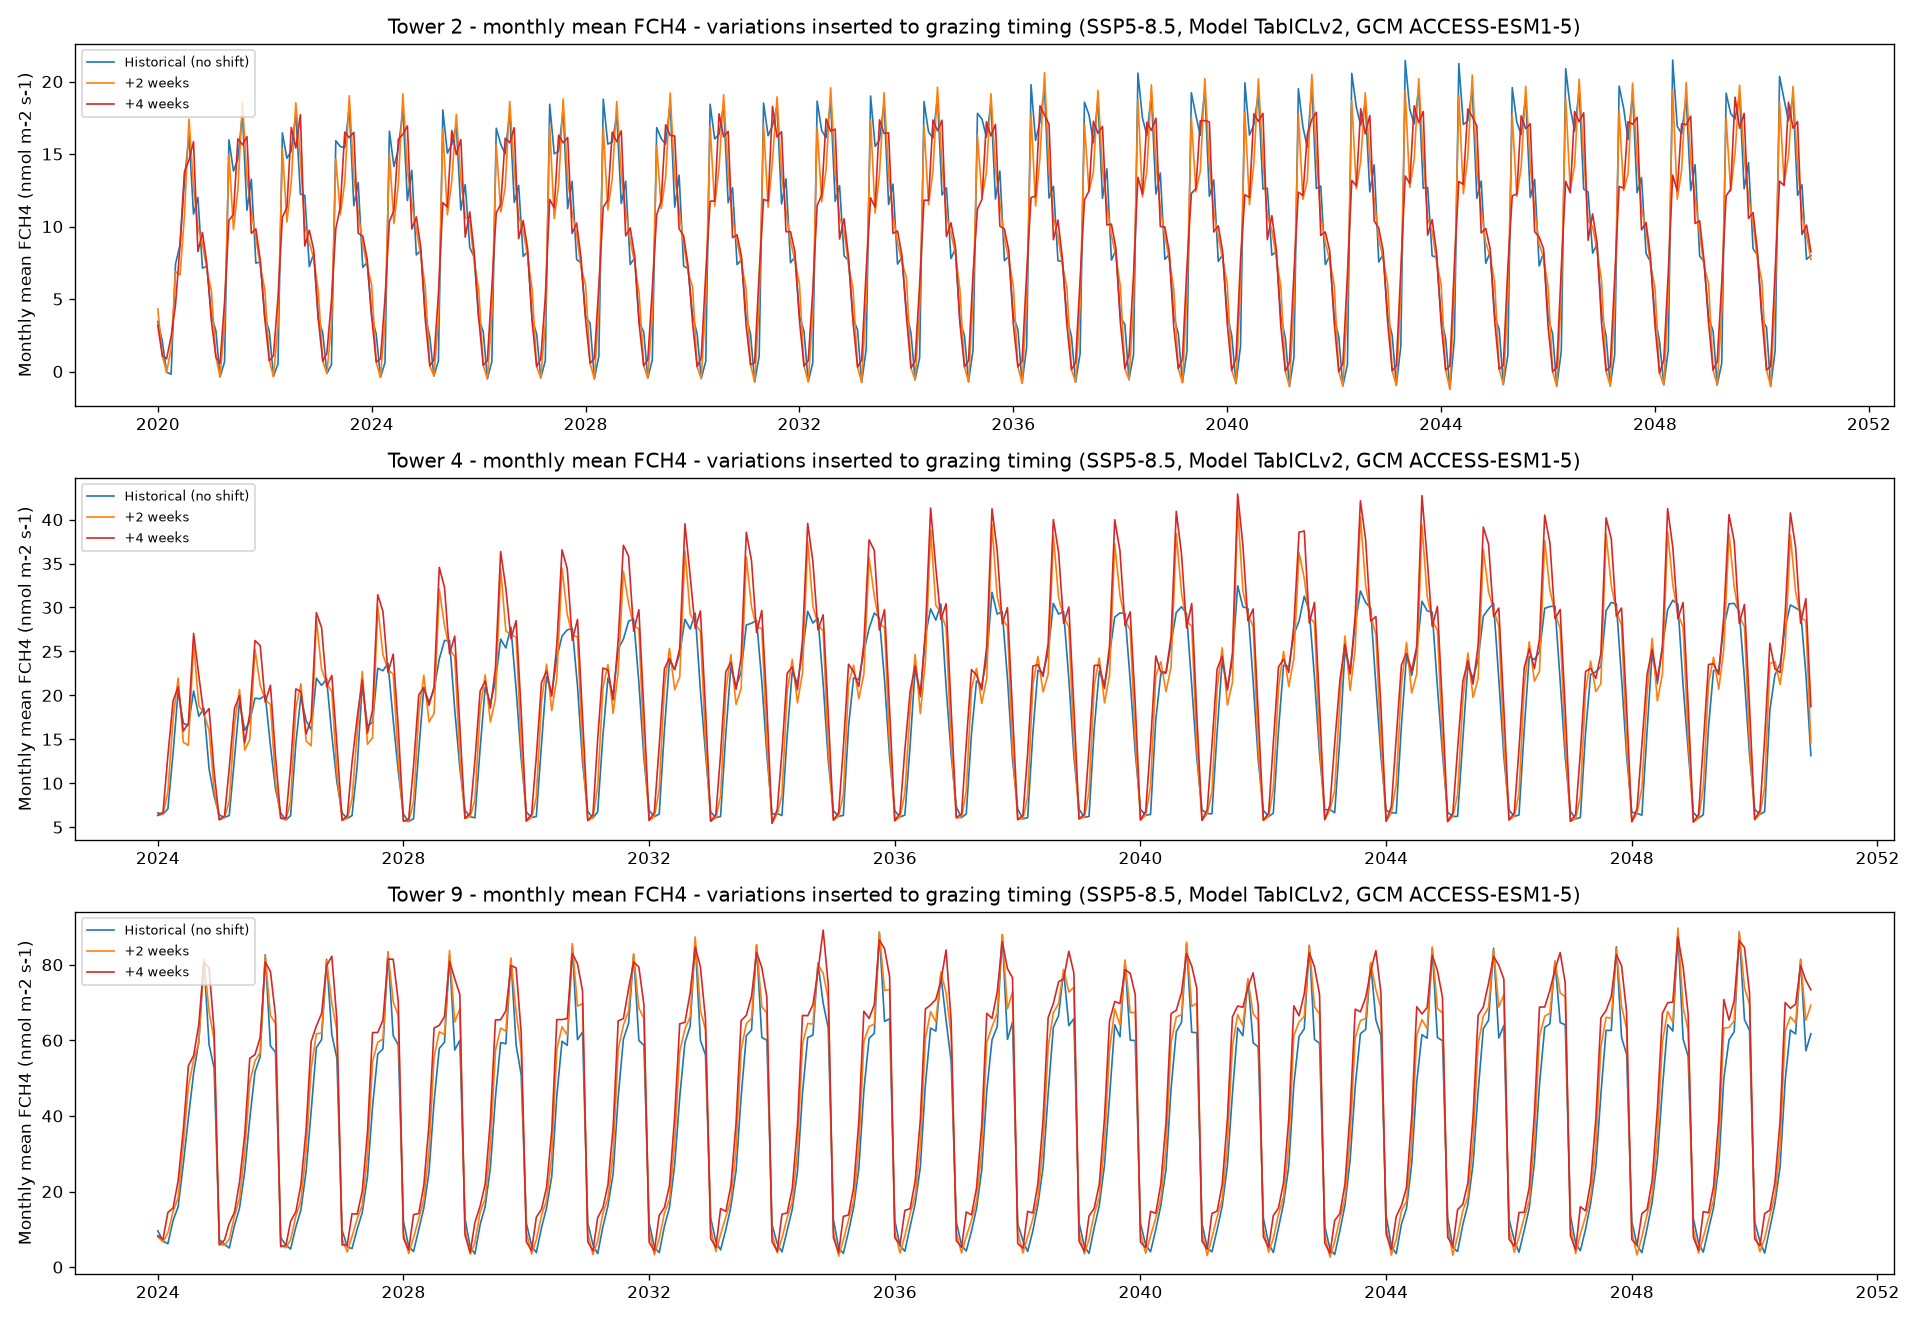
\includegraphics[width=\textwidth]{Figures/ch6_grazing_trajectory_ssp585.png}
\caption{
    Monthly mean FCH\textsubscript{4} (nmol~m\textsuperscript{-2}~s\textsuperscript{-1}) 
    at T2, T4 and T9 under SSP5-8.5 for the historical grazing-timing baseline and its
$+2$-week and $+4$-week shift perturbations, for a single illustrative trajectory
(restricted model, GCM ACCESS-ESM1-5, realisation~1). Table~\ref{tab:management_scenario_results} reports the mean
annual percentage change for the $+4$-week shift only, averaged across all five GCMs and ten
realisations per GCM.
}
\label{fig:app_sp_grazing_trajectory_ssp585}
\end{figure}

\FloatBarrier

\begin{figure}[htbp]
\centering
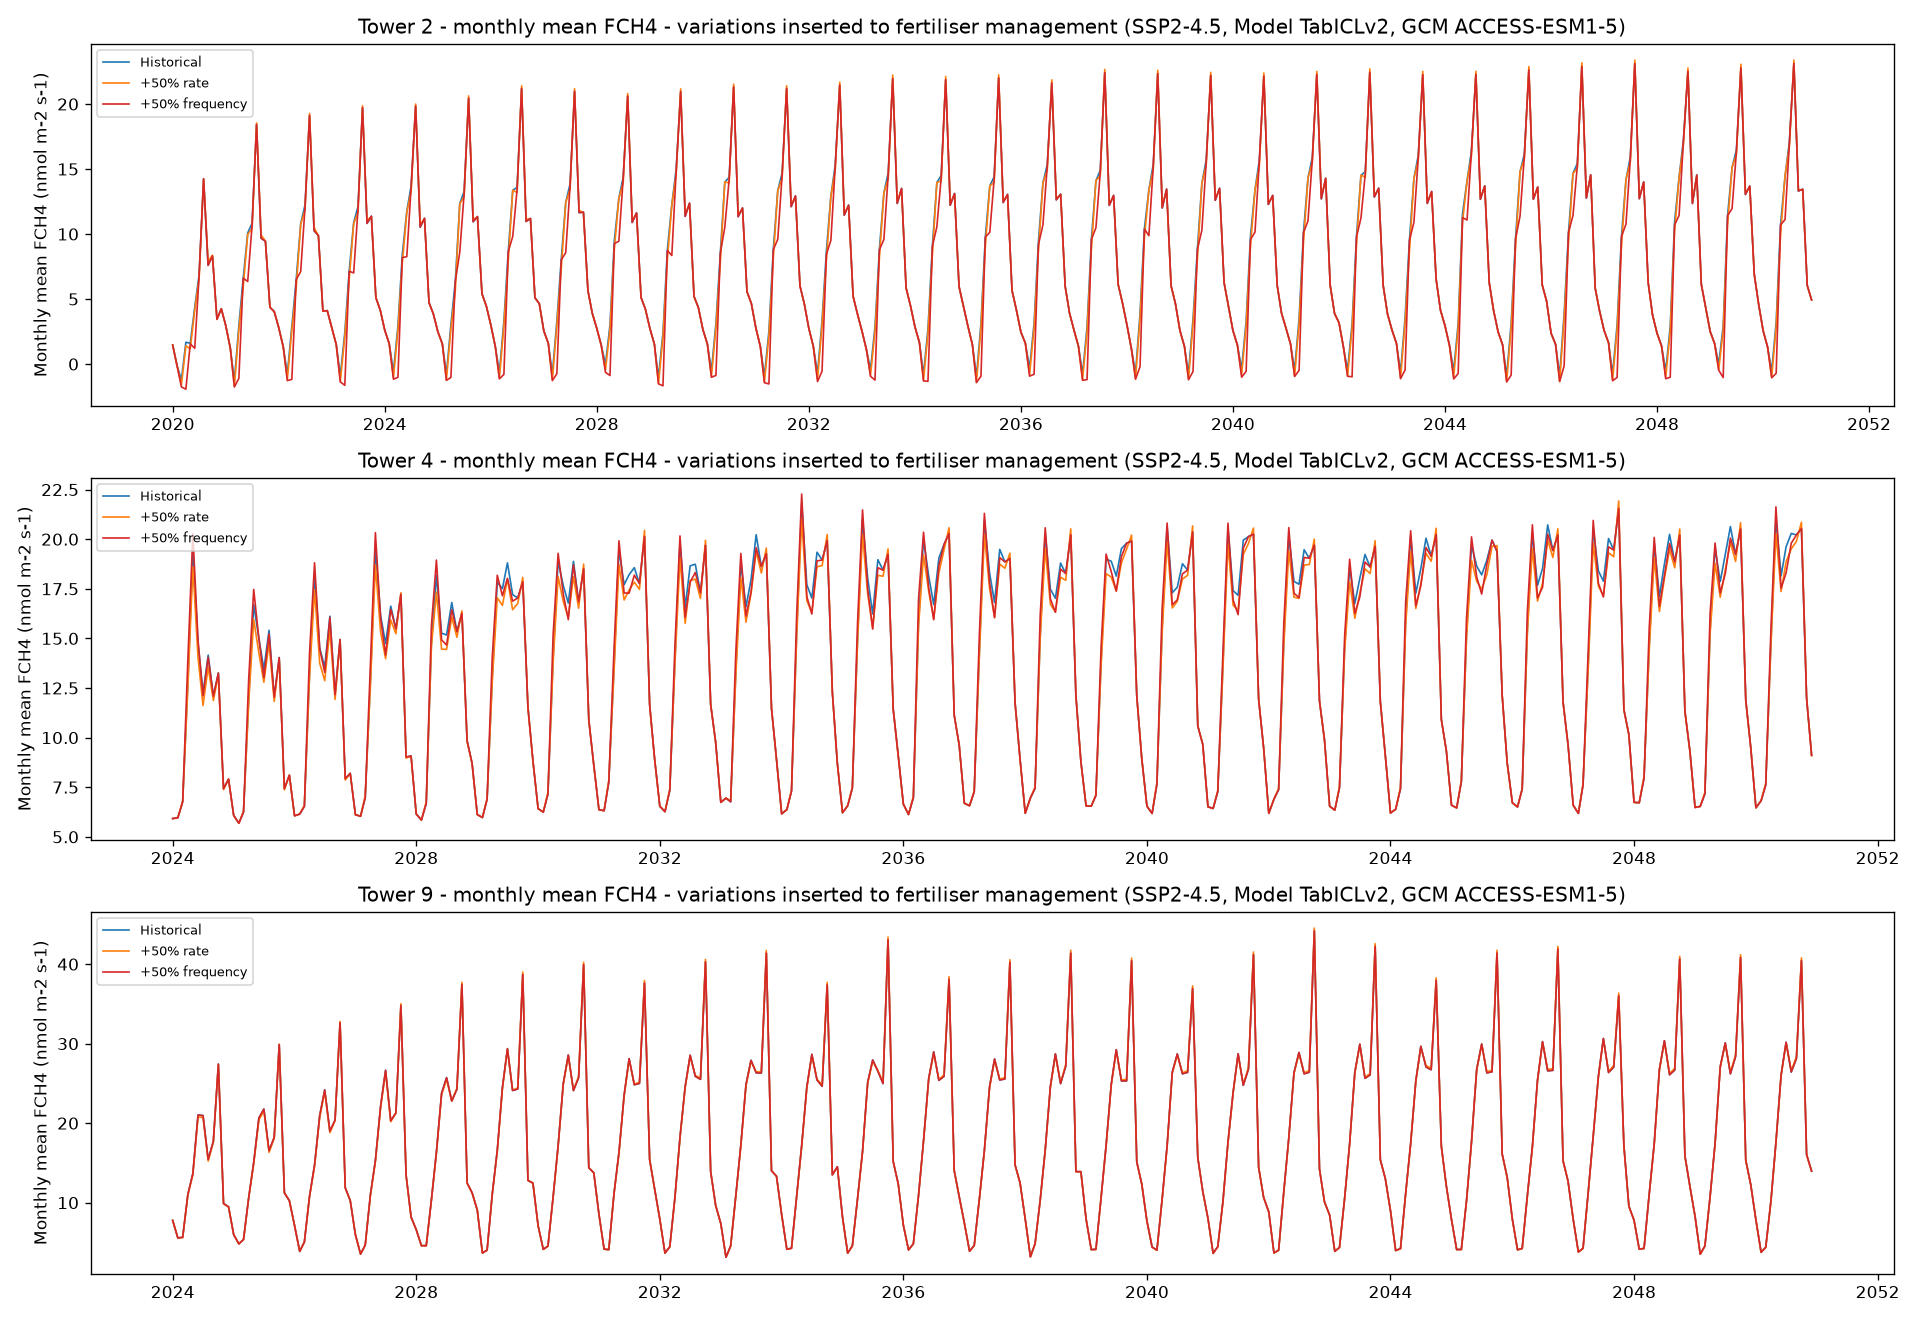
\includegraphics[width=\textwidth]{Figures/ch6_fertilizer_trajectory_ssp245.png}
\caption{
    Monthly mean FCH\textsubscript{4} (nmol~m\textsuperscript{-2}~s\textsuperscript{-1}) 
    at T2, T4 and T9 under SSP2-4.5 for the historical fertiliser-management baseline and its
$+50\%$-rate and $+50\%$-frequency perturbations, for a single illustrative trajectory
(restricted model, GCM ACCESS-ESM1-5, realisation~1). The three lines are visually near-identical
at every tower, consistent with Table~\ref{tab:management_scenario_results}'s finding that
fertiliser interventions produce only a small effect on predicted FCH\textsubscript{4}.
}
\label{fig:app_sp_fertilizer_trajectory_ssp245}
\end{figure}

\begin{figure}[htbp]
\centering
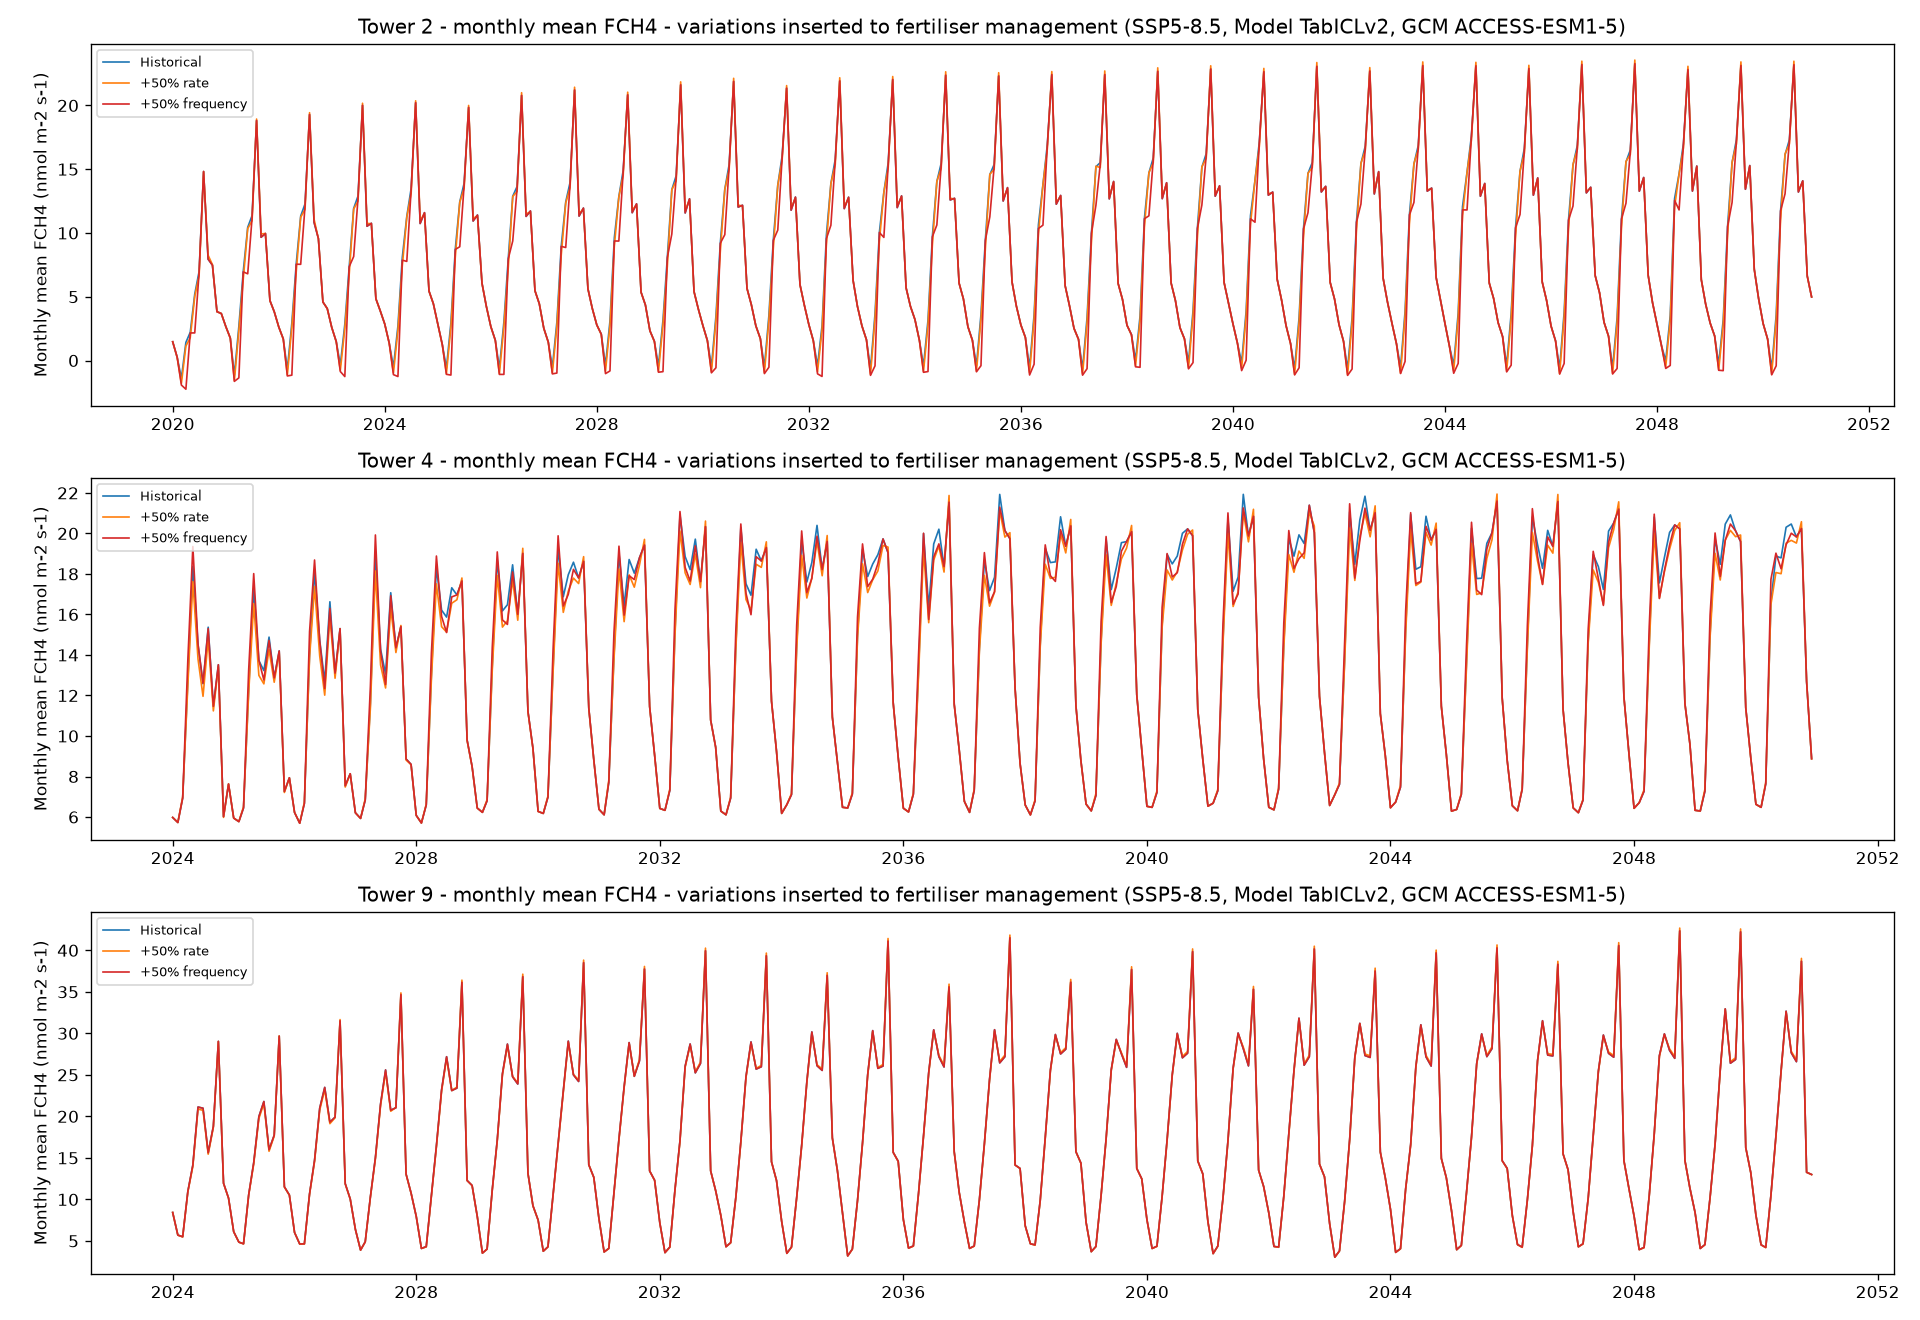
\includegraphics[width=\textwidth]{Figures/ch6_fertilizer_trajectory_ssp585.png}
\caption{
    Monthly mean FCH\textsubscript{4} (nmol~m\textsuperscript{-2}~s\textsuperscript{-1}) 
    at T2, T4 and T9 under SSP5-8.5 for the historical fertiliser-management baseline and its
$+50\%$-rate and $+50\%$-frequency perturbations, for a single illustrative trajectory
(restricted model, GCM ACCESS-ESM1-5, realisation~1). The three lines are visually near-identical
at every tower, consistent with Table~\ref{tab:management_scenario_results}'s finding that
fertiliser interventions produce only a small effect on predicted FCH\textsubscript{4}.
}
\label{fig:app_sp_fertilizer_trajectory_ssp585}
\end{figure}

\FloatBarrier
